\id{МРНТИ 50.01.01}{https://doi.org/10.58805/kazutb.v.2.27-1098}

\begin{articleheader}
\sectionwithauthors{Б.Қ. Нұрахметов, Ж.Т. Жұмашева}{СҰРЫПТАУ ЖӘНЕ ЖАРАМСЫЗ ДЕП ТАНУДЫҢ РОБОТТАНДЫРЫЛҒАН ЖҮЙЕСІН ЖАСАУ}

{\bfseries
\textsuperscript{1}Б.Қ. Нұрахметов\alink{https://orcid.org/0000-0002-5064-8687},
\textsuperscript{2}Ж.Т. Жұмашева\alink{https://orcid.org/0000-0001-7158-0995}\textsuperscript{\envelope }
}
\end{articleheader}

\begin{affiliation}
\textsuperscript{1}Алматы Технологиялық Университеті, Алматы, Қазақстан,

\textsuperscript{2}Әл-Фараби атындағы Қазақ Ұлттық Университеті, Алматы, Қазақстан

\raggedright \textsuperscript{\envelope }Корреспондент-автор: Zhadyra\_14@mail.ru
\end{affiliation}

Машиналық көру жүйелері бүгінде өнім сапасын қамтамасыз ету мәселесін
шешудің негізгі элементтерінің бірі болып табылады. Бұл геометриялық
өлшемді бақылау, дефектоскопия, сыртқы түрін бақылау, сұрыптау мен
жарамсыз деп тануды автоматтандыру, құрастыруды бақылау, орау сапасын
бақылау, белгілер мен белгілерді оқу және тану және т. б. Техникалық
көру және жасанды интеллектті пайдалана отырып сұрыптау технологиясы
оптикалық компоненттермен және жарықтандыру аспаптарымен үйлесімде
арнайы камераның көмегімен бұйымның (объектінің, дайындаманың,
бөлшектің) фотосуретін алу болып табылады. Соңғы уақытқа дейін өнімнің
сапасын бақылаудың жалғыз құралы өнімді тексеріп, оны жою немесе өткізіп
жіберу туралы шешім қабылдаған адам болды. Бүгінгі таңда өндіріс
желілерінде адамдар техникалық көру жүйелерін толығымен ауыстырды.
Жасанды интеллект және техникалық көру технологиялары өндіріс кезеңінде
дайын өнімді сұрыптау және жарамсыз деп тану операцияларында адамды
ауыстыруға мүмкіндік береді. Техникалық көру және жасанды интеллект
жүйелерін қолдану әр түрлі және қазіргі заманғы өнеркәсіптік өндірістің
барлық салаларын қамтиды, онда ағындық желілер бар. Тапсырмалар бойынша
жіктеу, ең алдымен, дәнекерлеу, бояу, жапсырма жапсыру және т.б. кезінде
сапаны бақылау және ақауларды жою. Жұмыстың мақсаты-компьютерлік көру
және жасанды интеллект құралдарының көмегімен өнімдерді сұрыптауды және
жарамсыз деп тануды жүзеге асыратын роботтандырылған жүйені құру. Бұл
жұмыста техникалық көру жүйесі мен контурды талдау жүйесі негізінде
өнімдерді сұрыптауды және жарамсыз деп тануды жүзеге асыратын
роботтандырылған жүйе жасалады. Роботтандырылған жүйе LabVIEW виртуалды
құралы мен Arduino UNO микроконтроллері негізінде жасалған.

{\bfseries Түйін сөздер:} бағдарлама, имитациялық модель, машиналық оқыту,
өнеркәсіптіқ робот, өнімді сұраптау.

\begin{articleheader}
{\bfseries РАЗРАБОТКА РОБОТИЗИРОВАННОЙ СИСТЕМЫ СОРТИРОВКИ И ОТБРАКОВКИ}

{\bfseries
\textsuperscript{1}Б.К. Нурахметов,
\textsuperscript{2}Ж.Т. Жумашева\textsuperscript{\envelope }
}
\end{articleheader}

\begin{affiliation}
\textsuperscript{1}Алматинский технологический университет, Алматы, Казахстан,

\textsuperscript{2}Казахский национальный университет им. аль-Фараби, Алматы, Казахстан,

e-mail: Zhadyra\_14@mail.ru
\end{affiliation}

Системы машинного зрения сегодня являются одними из ключевых элементов в
решении задачи обеспечения качества продукции. Это контроль
геометрических размеров, дефектоскопия, контроль внешнего вида,
автоматизация сортировки и отбраковки, контроль сборки, контроль
качества упаковки, считывание и распознавание меток и маркировок и т.п.

Технология сортировки с использованием технического зрения и
искусственного интеллекта заключается в получении фотографии изделия
(объекта, заготовки, детали) с помощью специальной камеры в комбинации с
оптическими компонентами и приборами освещения.

До недавнего времени единственным средством контроля качества продукции
был человек, который осматривал изделие и принимал решение о его
выбраковке или пропуске. Сегодня на линиях промышленности и производства
людей практически полностью заменили системы машинного зрения.

Технологии искусственного интеллекта и технического зрения дают
возможность заменить человека в операциях сортировки и отбраковки
готовых изделий на этапе производства.

Применение систем технического зрения и искусственного интеллекта
разнообразно и охватывает практически все сферы современного
промышленного производства, где есть поточные линии. Классифицируя по
задачам это, прежде всего, контроль качества и выбраковка брака при
сварке, окраске, наклейке этикеток и т.п. Также машинное зрение широко
используется при учете товаров.

Целью работы является создание роботизированной системы, осуществляющей
сортировку и отбраковку изделий с помощью инструментов машинного зрения
и искусственного интеллекта.

В данной работе разрабатывается роботизированная система, осуществляющая
сортировку и отбраковку изделий на основе системы технического зрения и
системы анализа контура. Роботизированная система выполнена на основе
виртуального прибора LabVIEW и микроконтроллера Arduino UNO.

{\bfseries Ключевые слова:} программа, имитационная модель, машинное обучение,
промышленный робот, сортировка изделий.

\begin{articleheader}
{\bfseries DEVELOPMENT OF A ROBOTIC SYSTEM FOR SORTING AND REJECTING}

{\bfseries
\textsuperscript{1}B.К. Nurakhmetov,
\textsuperscript{2}Zh.Т. Zhumasheva\textsuperscript{\envelope }
}
\end{articleheader}

\begin{affiliation}
\textsuperscript{1}Almaty Technological University, Almaty, Kazakhstan,

\textsuperscript{2}Kazakh National University named after Al-Farabi, Almaty, Kazakhstan,

e-mail: Zhadyra\_14@mail.ru
\end{affiliation}

Machine vision systems today are one of the key elements in solving the
problem of ensuring product quality. This is control of geometric
dimensions, flaw detection, appearance control, automation of sorting
and rejection, assembly control, packaging quality control, reading and
recognition of marks and markings, etc.

Sorting technology using machine vision and artificial intelligence
involves obtaining a photograph of a product (object, workpiece, part)
using a special camera in combination with optical components and
lighting devices.

Until recently, the only means of quality control of products was a
person who inspected the product and made a decision on its rejection or
passing. Today, people have been almost completely replaced by machine
vision systems on production lines.

Artificial intelligence and machine vision technologies make it possible
to replace people in sorting and rejection operations of finished
products at the production stage.

The use of machine vision and artificial intelligence systems is diverse
and covers almost all areas of modern industrial production where there
are flow lines. Classifying by tasks, this is, first of all, quality
control and rejection of defects during welding, painting, labeling,
etc. Machine vision is also widely used in accounting of goods.

The goal of the work is to create a robotic system that sorts and
rejects products using machine vision and artificial intelligence tools.

In this work, a robotic system is developed that sorts and rejects
products based on a machine vision system and a contour analysis system.
The robotic system is based on a LabVIEW virtual device and an Arduino
UNO microcontroller.

{\bfseries Keywords:} program, simulation model, machine learning,
industrial robot, sorting products.

\begin{multicols}{2}
{\bfseries Кіріспе.} Дайын бұйымдарды сұрыптау және жарамсыздандыру сияқты
процестерді автоматтандыру «адами факторды» болдырмайды және өнім
сапасының айтарлықтай жетілдірілуіне, өнімділіктің артуына және ақаудың
қысқаруына кепілдік береді {[}1{]}.

Машиналық көру - бұл жасанды интеллект, атап айтқанда, робототехника
саласындағы ғылыми бағыт және онымен байланысты нақты әлем
объектілерінің бейнелерін алу, оларды өңдеу және адамның қатысуынсыз
(толық немесе ішінара) әртүрлі қолданбалы міндеттерді шешу үшін алынған
деректерді пайдалану технологиялары.

Заманауи техникалық көру - қолданбалы ғылымның ең жылдам дамып келе
жатқан салаларының бірі. Техникалық көзқарас қағидаттарын пайдаланатын
жүйелер адам қызметінің әртүрлі салаларында кеңінен қолданылады.
Техникалық көзқарасты қолданудың ең танымал бағыттарының бірі
қоймалардағы қоқыстарды, құрылыс қалдықтарын және сақтау бірліктерін
сұрыптауға байланысты міндеттер болып табылады {[}2{]}.

Машина көруі өнеркәсіп пен өндіріс үшін компьютерлік көруді қолдану
болып табылады. Компьютерлiк көру - бұл компьютерлерге инженерлiк бағыт
ретiнде машиналық көру қызығушылығының аймағын көруге мүмкiндiк беретiн
әдiстердiң жалпы жиынтығы енгiзу-шығару сандық құрылғылары және ақаулы
өнiмдердi алуға арналған робот-манипуляторлар немесе аппараттар сияқты
өндiрiстiк жабдықтарды бақылауға арналған компьютерлiк желiлер болып
табылады. Машиналық көру есептеу техникасымен, оптикамен, машина
жасаумен және өнеркәсіптік автоматтандырумен байланысты инженерлік
бөлімше болып табылады.

Машинамен көрудің міндеттеріне:

- тану; - сәйкестендіру;

- табу; - мәтінді тану;

- 2D суреттер бойынша 3D пішінді қалпына келтіру;

- қозғалысты бағалау; - сахнаны қалпына келтіру;

- бейнелерді қалпына келтіру;

-кескіндердегі құрылымдардың белгілі бір түрін таңдау, кескіндерді
сегменттеу;

- оптикалық ағынды талдау.

Компьютерлік көру саласы жас, әртүрлі және серпінді дамып келе жатқан
ретінде сипатталуы мүмкін.

Жасанды интеллект саласындағы маңызды бөлікті автоматты жоспарлау немесе
роботты кейбір ортадан өткізу сияқты механикалық әрекеттерді орындай
алатын жүйелерде шешім қабылдау алады. Өңдеудің бұл түрі әдетте
бейнесенсор ретінде әрекет ететін және орта мен робот туралы жоғары
деңгейлі ақпарат беретін компьютерлік көру жүйелері ұсынатын кіріс
деректерін қажет етеді.

Аталған талаптарды деректерді өңдеудің белгілі математикалық әдістерін
пайдалануға мүмкіндік беретін NI LabVIEW - қосымшаларды әзірлеудің
графикалық ортасына негізделген National Instruments (NI) компаниясының
шешімдері қанағаттандырады. NI IMAQ Vision қосымша техникалық көру
модулі аналогтық және сандық көздерден бейнелерді жүктеуге мүмкіндік
береді, көптеген талдау және бейнелерді өңдеу функцияларына ие.
Бейнелерді алудың меншікті аппараттық құралдарынан басқа, NI жоғары
шешімді сандық камераларды (СК) қоса алғанда, бөгде өндірушілердің
көздерінен деректер жинай алады. NI LabVIEW әзірлеу ортасы модульдік
және иерархиялық, бұл NI қосымша модульдерінде ұсынылған математикалық
әдістердің функцияларын пайдалануға мүмкіндік береді. Мысалы, NI
Advanced Signal Processing Toolkit модулі {[}3{]}.

Арнайы бағдарламалық қамтамасыз етудің қолдауымен компьютерлік талдау
орындалады және бейнені өңдеу, бұдан әрі өнімнің қандай да бір сыныпқа
жататындығы, өнімнің жарамдылығы/жарамсыздығы туралы қорытынды автоматты
түрде жасалады не адамның қабылдауына ыңғайлы нысанда бұйымды зерделеу
қорытындылары туралы есеп жасалады (сурет 1).

Техникалық көрудің автоматтандырылған жүйесі жұмысының негізгі
элементтерінің бірі сегменттеу болып табылады, өйткені дәл осы өңдеу
кезеңінде объектілер одан әрі тану және талдау үшін сахнадан бөлінеді.
Кескінді сегменттеу кескінді олардың нүктелеріндегі сипаттардың
(белгілердің) ұқсастығы бойынша аумаққа бөлуді білдіреді. Бейнелерді
сегменттеудің негізгі түрлеріне жарықтылық, түсті координаттар,
контурлар, пішін бойынша сегменттеу жатады {[}4,5{]}. Сегменттеу түрлері
туралы білімдерге сүйене отырып, кескіндерді сегменттеудің әртүрлі
әдістерін бөліп көрсетуге болады: - облыстарды өсiру әдiсiмен сегменттеу
- пикселдердi немесе iрi қалыптарды алдын ала берiлген өсу өлшемдеріне;
- бөлу әдісімен сегменттеу - кескін кейбір өлшемшарттардың көмегімен
қиылыспайтын блоктарға бөлінеді, біртектілігі тексеріледі; - бейнелердің
амплитудалық түрлендірулері - бұл бейнедегі элементтердің мәндерін
өзгертетін алгоритмдер; - суретті сүзу (негізінен, бұл белгілі бір
ядромен орау алгоритмдері).
\end{multicols}

\begin{figure}[H]
	\centering
	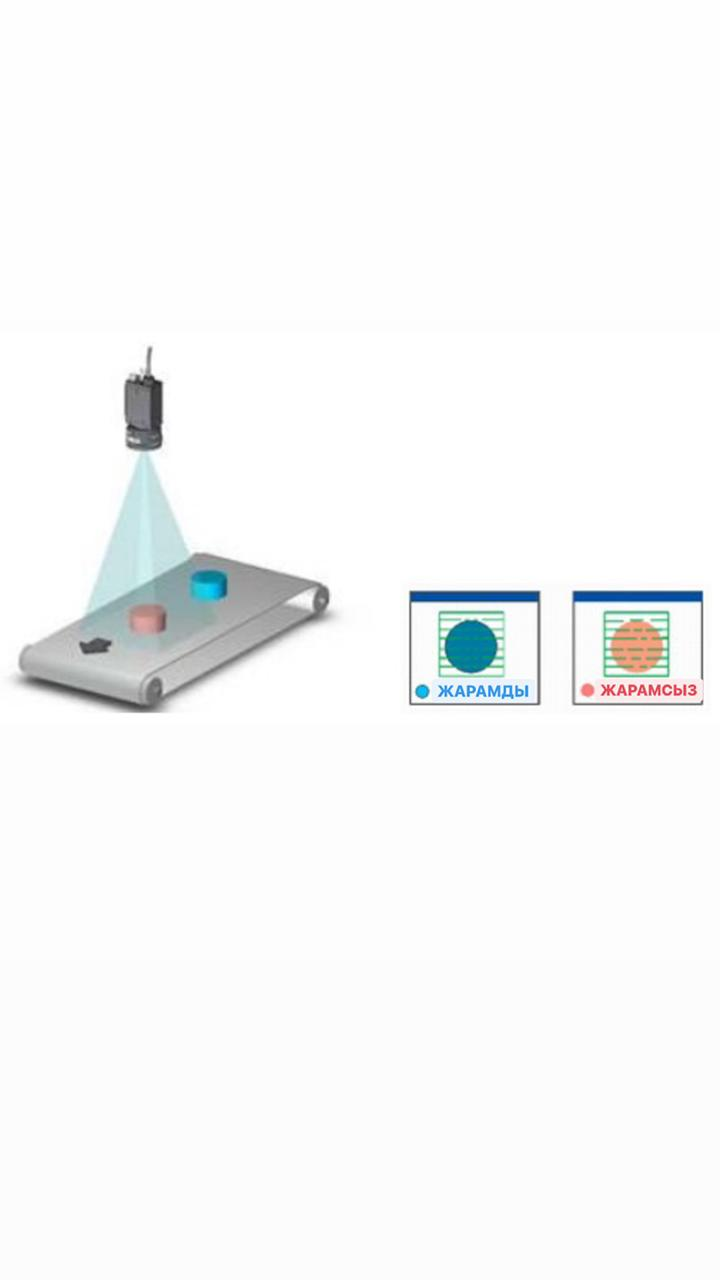
\includegraphics[width=0.5\textwidth]{media/ict2/image168}
	\caption*{1 - сурет. Бейнекамераның көмегімен конвейерде автоматты сұрыптау үрдісінің жалпы көрінісі}

\end{figure}

\begin{multicols}{2}
Сұрыптаудың қолданыстағы өндірістік жүйелері. KUKA \_3D Perception
стерео сенсоры.3D стереокамералар жүйесі орнатылған сенсор нақты уақыт
режімінде 3D-қабылдауды жүзеге асыруға мүмкіндік береді және кеңістікте
3D өлшеу мен орналастыруды қамтамасыз етеді. Осылайша, кеңістіктегі
бағдарлау және техникалық көру шындыққа айналады (сурет 2) {[}6{]}.
\end{multicols}

\begin{figure}[H]
	\centering
	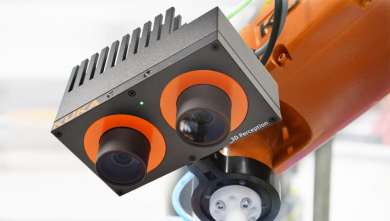
\includegraphics[width=0.6\textwidth]{media/ict2/image169}
	\caption*{2 - сурет. KUKA \_3D Perception стерео сенсоры}
\end{figure}

\begin{multicols}{2}
FANUC iRVision жүйесі. iRVision - FANUC компаниясы әзірлеген plug \&
play технологиясы бойынша визуалды анықтау жүйесі. Екі немесе үш өлшемді
бөлшектерді тану жүйесінің арқасында ол кез келген нысандағы және
өлшемдегі еркін орналасқан бұйымдардың орналасқан жерін анықтай алады.
Ол сондай-ақ штрихкодтарды оқи алады, түс бойынша сұрыптауды,
бөлшектердің икемді берілуін, жоғары жылдамдықты визуалды сызықтық
қадағалауды (iRPickTool) және қораптарды/панельдерді ала алады. iRVision
жүйесі өнімділікті арттыруда негізгі рөл атқарады және қосымша қаражатты
үнемдеуді қамтамасыз етеді, өйткені ол технологиялық жабдықтың
қажеттілігін жояды (сурет 3).
\end{multicols}

\begin{figure}[H]
	\centering
	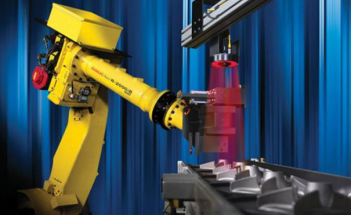
\includegraphics[width=0.6\textwidth]{media/ict2/image170}
	\caption*{3 - сурет. iRVision жүйесі}
\end{figure}

\begin{multicols}{2}
Baumer CX IP 65/67 машиналық көру камералары жабдықтың осы сыныбына
арналған бірегей ерекшеліктерге ие. Олар қаптаманың көмегімен қосымша
қорғаудың қажеттілігінсіз қоршаған ортаның күрделі жағдайларындағы ең
талап етуші қолданыстарда пайдаланылуы мүмкін. IP 65/67 корпусының
арқасында камералар су мен шаңнан сенімді қорғалған (сурет 4).
\end{multicols}

\begin{figure}[H]
    \centering
    \begin{subfigure}[t]{0.35\textwidth}
        \centering
        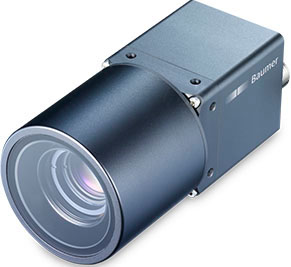
\includegraphics[width=\textwidth]{media/ict2/image171}
    \end{subfigure}
    \begin{subfigure}[t]{0.35\textwidth}
        \centering
        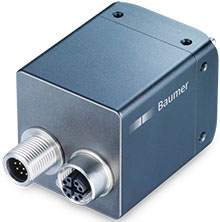
\includegraphics[width=\textwidth]{media/ict2/image172}
    \end{subfigure}
    \caption*{4 - сурет. Baumer CX IP 65/67 камералары}
\end{figure}

\begin{multicols}{2}
{\bfseries Материалдар және әдістер.}LabVIEW (National Instruments) -
әртүрлі енгізу/шығару құрылғыларынан деректерді жинауды, өңдеуді және
визуализациялауды орындайтын виртуалды аспаптарды жасауға мүмкіндік
беретін бағдарламаларды әзірлеуге және орындауға арналған бағдарламалық
қамтамасыз ету. Осы бағдарламалық қамтамасыз етудің басты ерекшелігі
оның бағдарламалау тілі - деректер ағындарының архитектурасына
негізделген «G» графикалық тілі болып табылады {[}7-9{]}.

LabVIEW бағдарламалық қамтамасыз ету базасындағы виртуалды құрал
камерадан бейнелер жинауды жүзеге асырады, оларды арнайы алгоритмдер
негізінде өңдейді, бұйымның ақау дәрежесін талдайды және өз жұмысының
нәтижелерін визуализациялайды.

Сұрыптау жүйесінің аппараттық бөлігі ретінде Arduino UNO
микроконтроллері әрекет етеді. Arduino Uno - ATmega328P-AU процессоры
негізінде жасалған контроллер. Оның құрамына процессордан басқа: 16
сандық контактілер, 6 аналогтық контактілер, 16 МГц кварц резонаторы,
USB қосқышы, қуат қосқышы, ICSP ішкі схемалық бағдарламалау қосқышы,
шығару түймесі кіреді. USB-UART түрлендіргіші ретінде ATmega16U2
микроконтроллері қолданылады. Элементтердің платада орналасуы 5-суретте
көрсетілген.
\end{multicols}

\begin{figure}[H]
	\centering
	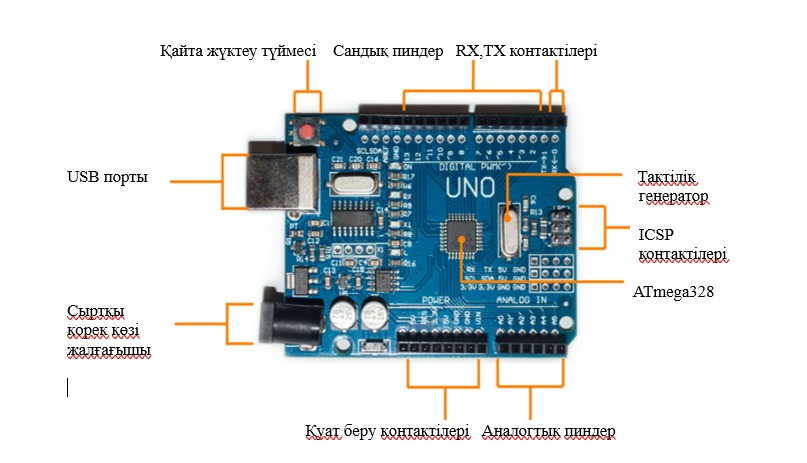
\includegraphics[width=0.6\textwidth]{media/ict2/image173}
	\caption*{5 - сурет. Контроллер элементтерінің орналасуы}
\end{figure}

\begin{multicols}{2}
Микроконтроллермен қоректендіру әртүрлі көздерден келеді: - компьютерден
немесе басқа құрылғыдан USB порты арқылы; - DC 2.1 қосқышы арқылы сыртқы
адаптерден; - GND және VIN байланыстары арқылы батареядан.

Қуат көзі автоматты түрде таңдалады. Қоректендіру кернеуінің ұсынылған
диапазоны 7-12 В.
\end{multicols}

\tcap{1 - кесте. Контроллердің негізгі сипаттамалары}
\begin{longtblr}[
  label = none,
  entry = none,
]{
  cells = {c},
  hlines,
  vlines,
}
\textbf{Сипаттамасы} & \textbf{Мәні}\\
Жұмыс
			кернеуі & 5,0
			В\\
Ұсынылатын
			кіріс кернеуі & 7,0
			В … 12,0 В\\
Шекті
			кіру кернеуі & 6,0
			В … 20,0 В\\
Цифрлық
			байланыстардың саны & 14
			(6 ШИМ)\\
Ұқсас
			контактілер саны & 6\\
Енгізу/шығару
			түйіспелерінің тоғы & 40
			мА\\
Флэш-жад
			32 Кб & 32
			Кб\\
SRAM-жады
			(энергияға тәуелді) & 2
			Кб\\
EEPROM-жады
			(энергияға тәуелсіз) & 1
			Кб\\
Тактілік
			жиілігі & 16
			МГц\\
Төлем
			мөлшері & 70мм
			х 53мм
\end{longtblr}

6-суретте деректерді енгізу/шығарудың барлық сандық және аналогты
контактілері белгіленген.

\begin{figure}[H]
	\centering
	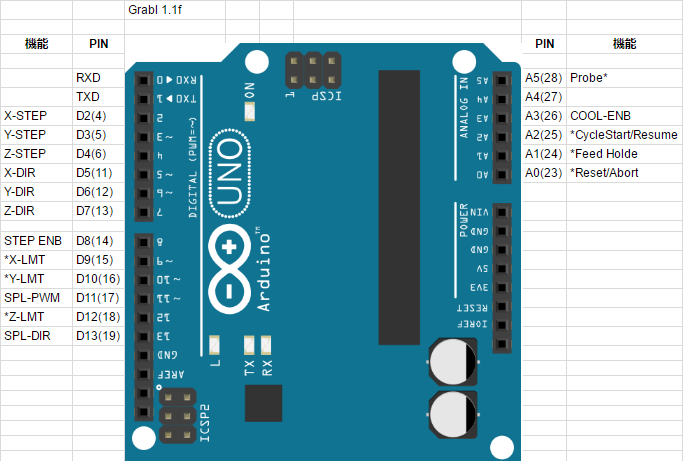
\includegraphics[width=0.6\textwidth]{media/ict2/image174}
	\caption*{6 - сурет. Контроллердің сандық және аналогтық контактілері}
\end{figure}

\begin{multicols}{2}
Таңдалған контроллер кеңейтілген RISC-сәулеті және төмен энергия тұтынуы
бар өнімді сегіз разрядты ATmega328P-AU микроконтроллерімен
жабдықталған.2-кестеде ATmega328P микроконтроллерінің негізгі
сипаттамалары берілген.
\end{multicols}

\tcap{2 - кесте. ATmega328P негізгі сипаттамалары}
\begin{longtblr}[
  label = none,
  entry = none,
]{
  cells = {c},
  hlines,
  vlines,
}
\textbf{Сипаттамасы} & \textbf{Мәні}\\
Қуат
			кернеуі & 1,8В
			… 5,5В\\
Жұмыс
			режимінде тұтынылатын ток & 0,2
			мА\\
Күту
			режимінде тұтынылатын ток & 0,75
			мкА\\
Тактілік
			жиілік & 20
			МГц\\
Flash
			жады & 32
			Кб\\
SRAM
			жады & 2
			Кб\\
EEPROM
			жады & 1
			Кб\\
Барлық
			порттар саны (ШИМ порттары) & 23(6)\\
АСТ
			арналарының саны & 6\\
АСТ
			рұқсаты & 10
			бит\\
8-разрядты
			санауыштар саны & 2\\
16-разрядты
			санауыштар саны & 1\\
Жалпы
			мақсаттағы тіркелімдер саны & 32х8
\end{longtblr}

\begin{multicols}{2}
SRAM-жады (2 Кб) энергияға тәуелді және шын мәнінде уақытша деректерді
сақтау үшін пайдаланылатын микроконтроллердің жедел жады болып табылады.
Деректерді ұзақ уақыт сақтау үшін энергияға тәуелсіз EEPROM-жады (1Кб)
бар. Сондай-ақ, микроконтроллер 32 Кб Flesh-жадымен жабдықталған, оның
ішінде 2 Кб құрылғыны USB порты арқылы тігуге мүмкіндік беретін
жүктегішке бөлінген.

Контроллердің бағдарламалық қамтамасыз етуі бағдарламаларды жазу және
оларды құрастыру үшін пайдаланылатын Arduino IDE бағдарламалық қабықшасы
болып табылады.

{\bfseries Нәтижелер және талқылау.} Бұл жұмыста LabVIEW {[}10{]} виртуалды
құралы, контроллер және аппараттық құралдар бір-бірімен байланыста жұмыс
істейді. Бұл жұмыс мынадай кезеңдердің бірізділігімен сипатталады:

а) камера тексеруді талап ететін бұйымдардың түсірілімдерін жүзеге
асырады және оларды компьютердің қатты дискісіндегі папкаға сақтайды;

б) осы компьютерде орнатылған виртуалды құрал осы суреттерге қол жеткізе
алады;

в) виртуалды аспап суреттерді өңдейді және бейненің контурын талдау
негізінде ақау дәрежесін анықтайды;

г) виртуалды құрал талдау нәтижесін визуализациялайды және тексеру
нәтижесін микроконтроллерге жібереді. Тексеру нәтижесі 2 түрлі болуы
мүмкін: теріс және жартылай қайталанатын;

д) бұл сигналды алғаннан кейін микроконтроллер өзінің қорытындыларында
цифрлық басқару сигналдарын қалыптастырады;

е) микроконтроллердің цифрлық сигналдары қандай да бір іс-қимылдарды
орындау үшін роботталған аппараттық құралдармен пайдаланылуы мүмкін. Бұл
жоба жағдайында екі жарық диодтары арқылы тексеру нәтижесі туралы дабыл
беріледі;

ж) виртуалды аспап камераның келесі түсірілімін талдайды. Талдау
секундына бір рет жүргізіледі.

Жүйе LabVIEW виртуалды құралының орындалуы мәжбүрлі тоқтатылғанға дейін
шексіз цикл режимінде жұмыс істейді.7-суретте камераның, дербес
компьютердің, виртуалды аспаптың және бақылаушының өзара іс-қимыл
сұлбасы көрсетілген.
\end{multicols}

\begin{figure}[H]
	\centering
	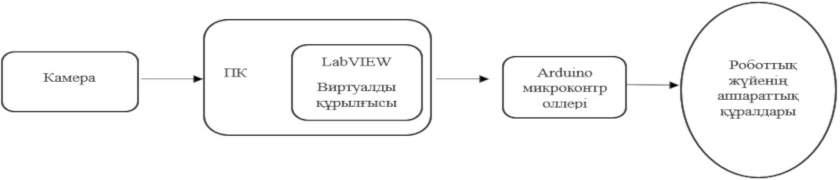
\includegraphics[width=0.8\textwidth]{media/ict2/image175}
	\caption*{7 - сурет. Роботтандырылған жүйенің құрылымдық сұлбасы}
\end{figure}

\begin{multicols}{2}
2.2 Әзірленген жүйенің сипаттамасы

Виртуалды құрал дербес компьютерге орнатылады және роботтандырылған
жүйенің зияткерлік бөлігі ғана емес, оның интерфейсі де болып табылады.

Бет панелінде аспапты басқару элементтері мен деректерді визуализациялау
элементтері бар.

Бет панелінде ақауға тексеруден өтетін бөлшектің бейнесі көрсетіледі.
Тексеру бұйымның күтілетін контурын нақты контурмен салыстыру арқылы
жүзеге асырылады. Виртуалды құрал осы екі контурдың айырмашылығын
өлшейді (суретте көк және жасыл контурлар).

Кестеде нақты контурдың күтілгеннен ауытқу шамасы көрсетілген. «Ақаудың
бақылау шамасы» басқару элементінің көмегімен бұйымдарды жарамсыз деп
табудың дәлдігін анықтауға болады. Егер нақты контурдың ауытқуы берілген
мәннен асып кетсе, бұйым ақау болып саналады және «Тексеру мәртебесі»
индикаторы қызыл түспен жанады. Сондай-ақ бөлшектің бейнесінде ақау
орындары қызыл түспен белгіленеді.

«Сериялық порт» элементі деректер бақылаушыға берілетін портты таңдау
үшін қажет. «Тоқта» түймешігі виртуалды құрылғыны тоқтатады.

8-суретте бұйымның ақауын анықтаған виртуалды аспаптың бет панелінің
сыртқы көрінісі көрсетілген.
\end{multicols}

\begin{figure}[H]
	\centering
	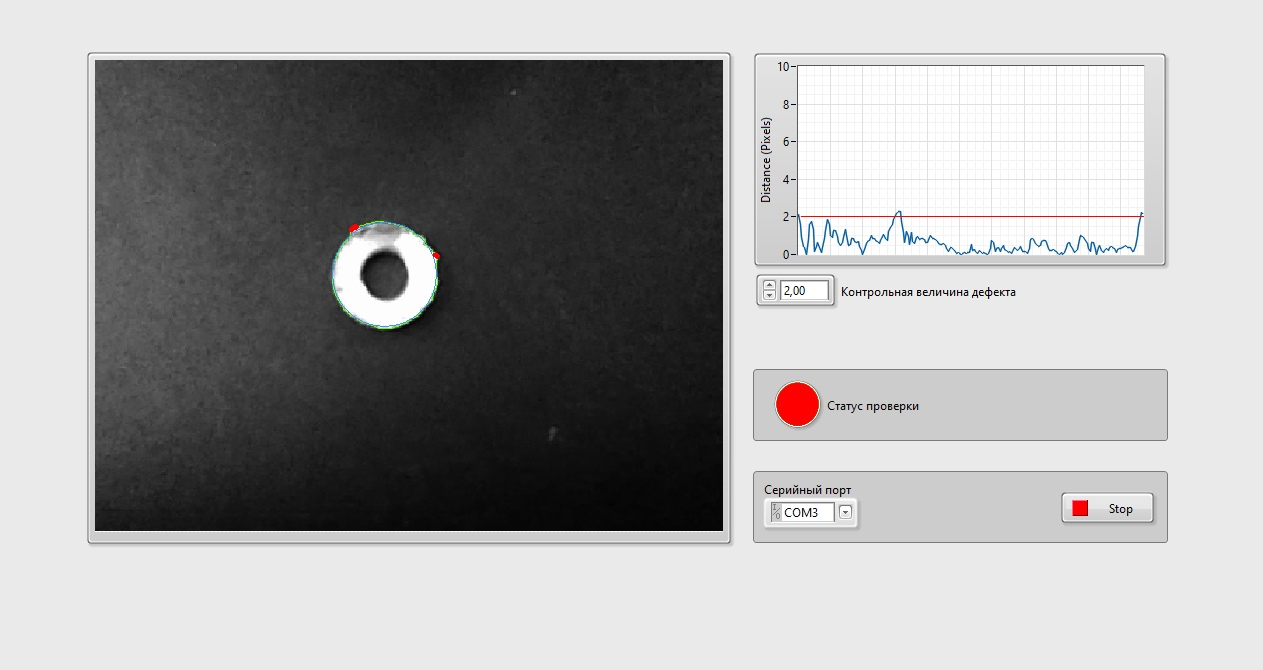
\includegraphics[width=0.75\textwidth]{media/ict2/image176}
	\caption*{8 - сурет. Виртуалды аспаптың бет панелі}
\end{figure}

9-суретте бұйымның ақауын анықтамаған виртуалды аспаптың бет панелінің
сыртқы көрінісі көрсетілген. Бұл бұйым рұқсат қағазын алады.

\begin{figure}[H]
	\centering
	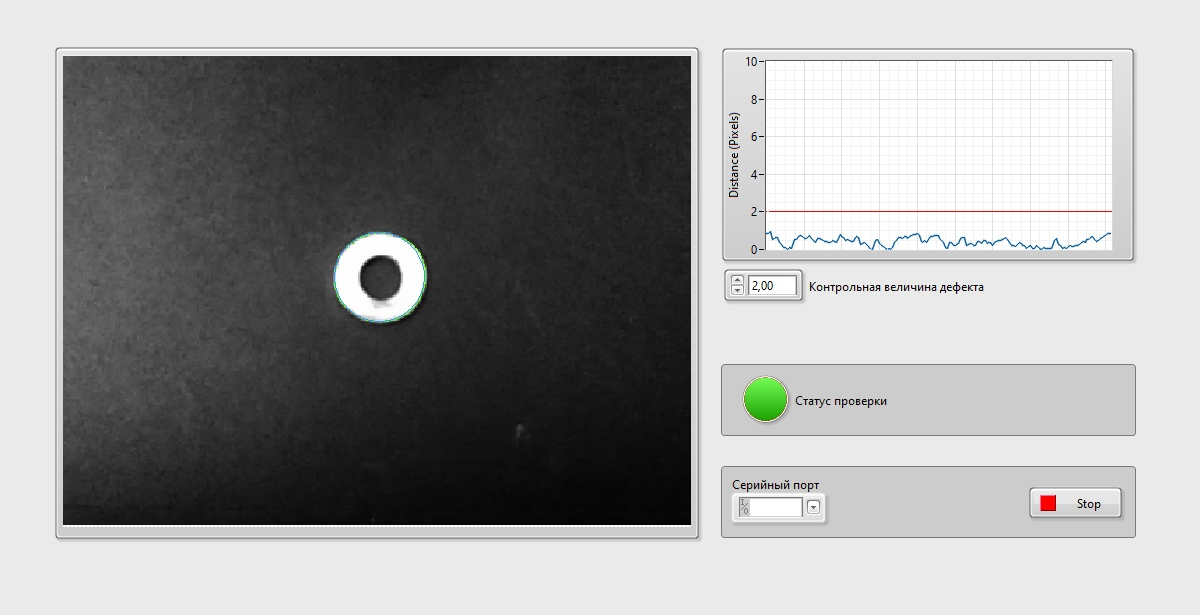
\includegraphics[width=0.75\textwidth]{media/ict2/image177}
	\caption*{9 - сурет. Виртуалды аспаптың бет панелі}
\end{figure}

\begin{figure}[H]
	\centering
	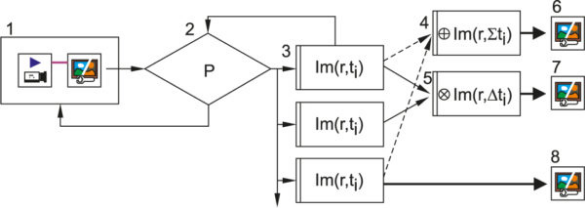
\includegraphics[width=0.7\textwidth]{media/ict2/image178}
	\caption*{10-сурет. Суреттер сериясын уақытша өңдеу жүйесінің құрылымы}
\end{figure}

\begin{multicols}{2}
Суреттердің қандай да бір жиынтығын алғаннан кейін оларды өңдеу міндеті
туындайды. Бұл үшін кейіннен өңдеу үшін олардың қолжетімділігін
қамтамасыз ете отырып, пайда болатын суреттермен буферді бағдарламалық
толтыруға болады. Жүйенің мұндай құрылымы 10-суретте көрсетілген.
Бейнелерді алу кезінде уақытша тактілеу жолымен және қажетті триггерлік
оқиғаның (P) көмегімен бейнелер сериясы қалыптастырылады. Содан кейін ол
буферге (3) толтырылады, ол бірлесіп алдын ала өңдеу үшін пайдаланылады:
сапа мен рұқсатты арттыру (4), бейнелерді жұптық корреляциялық талдау
(5). Нәтижесінде алынған бейнелерден (6-8) бақылау объектісі туралы
ақпараттық құрамдас бөліктер алынады.

Күрделі нысандар суретіндегі ішкі элементтердің құрылымы мен
көрсеткіштерін анықтау үшін берілген үлгілерді суреттердегі іздеуге
қолдануға болады: геометриялық, түсті және т.б. Бейнелерді талдаудың
мұндай функциялары 11-суретте берілген.
\end{multicols}

\begin{figure}[H]
	\centering
	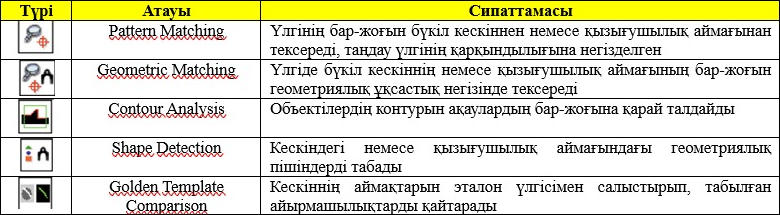
\includegraphics[width=0.8\textwidth]{media/ict2/image179}
	\caption*{11-сурет. Бейнелерді талдау функциялары}
\end{figure}

\begin{figure}[H]
	\centering
	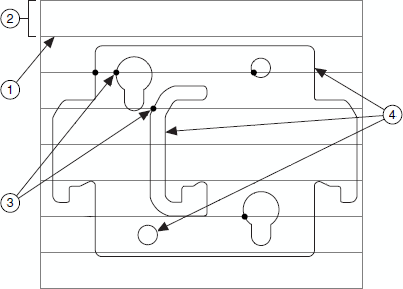
\includegraphics[width=0.6\textwidth]{media/ict2/image180}
	\caption*{12 - сурет. Контур қисығын анықтау процесі}
\end{figure}

\begin{multicols}{2}
Бұл жұмыста суреттер контурын талдау функциялары пайдаланылады.
Контурлар әдетте суреттегі бөлшектердің шекарасын білдіреді. Контур
қисықтары - бұл бақылау суретіндегі үлгіге сәйкестікті анықтау үшін
пайдаланылатын негізгі ақпарат.

Контур қисығын алу үдерісі қисықтың бастапқы нүктелерін іздеуден және
қисықты қадағалаудан тұрады.

Контурдың бастапқы нүктесі контурдың трассировкасы басталатын қисықтағы
нүкте болып табылады. Бастапқы нүкте ретінде саралау үшін пиксель
бұрыннан бар қисықтың бөлігі бола алмайды және шекті мәннен жоғары шеткі
контрасты болуы тиіс. Шеткі қарама-қарсылық бірінші бастапқы пикселден
бастап есептеледі. Егер шеттің қарама-қайшылығы берілген шектен үлкен
болса, қисық сызық осы нүктеден бастап трассаланады. Егер
қарама-қарсылық шектен төмен болса немесе бұл пиксель бұрыннан
есептелген қисықтың мүшесі болып табылса, алгоритм оның бастапқы нүкте
ретінде сәйкес келетінін анықтау үшін жолдағы келесі пиксельді талдайды.
Бұл процесс қисықты іздеу аймағының қарама-қарсы жағына қол жеткізгенге
дейін қайталанады. Содан кейін алгоритм процесті қайталайды.

Қисықты қадағалау (трассировка) - бұл қисықтағы соңғы пикселмен көршілес
пиксель осы қисыққа қосылатын процесс. Бұл үрдіс ағымдық бағыттағы
қисыққа пиксельдер қосылғанша қайталанады. Содан кейін алгоритм бастапқы
нүктеге оралады және қисықты кері бағытта бақылауға тырысады (12-сурет).

Блок-сұлбада контурды іздеу алгоритмін іске асыру үшін мынадай LabVIEW
құралдары пайдаланылады: IMAQ Extract Contour VI, IMAQ Fit Contour VI,
IMAQ Compute Contour Distances VI және IMAQ Overlay Contour VI. Бұл
қосалқы құралдар бейненің контурын алады, оны шаблондық контурмен
салыстырады және осы екі контурдың сәйкессіздік дәрежесін есептейді. Бұл
сәйкессіздік бұйымда ақаудың бар екенін куәландырады.

Кескіндерді өңдеу алдында осы кескіндерді алу қажет. Бұл үшін LabVIEW
Vision Acquisition Express VI арнайы бағдарламалық жасақтамасы
пайдаланылады, ол 13-суретте көрсетілген
\end{multicols}

\begin{figure}[H]
	\centering
	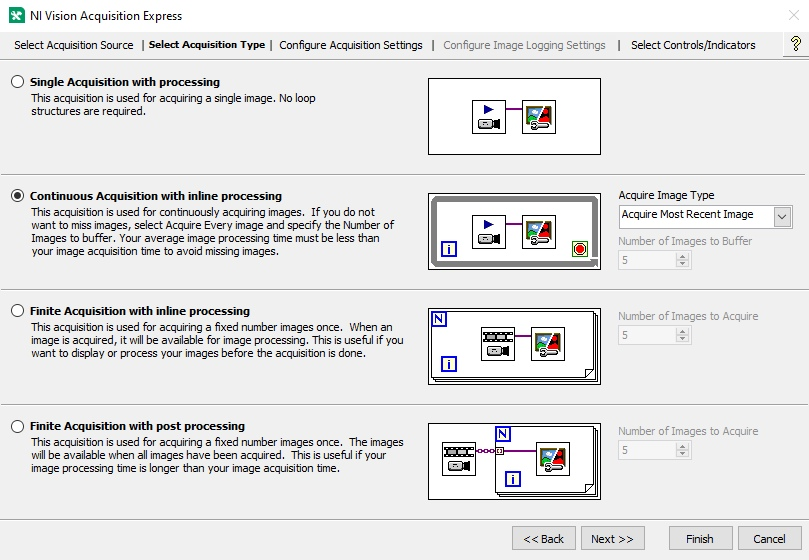
\includegraphics[width=\textwidth]{media/ict2/image181}
	\caption*{13-сурет. Виртуалды аспаптың блок сұлбасы}
\end{figure}

\begin{multicols}{2}
14-суретте деректерді жинау мен өңдеудің шексіз циклі болып табылатын
виртуалды аспаптың жалпы блок-сұлбасы көрсетілген.15-суретте бейненің
контурымен жұмыс істейтін қосалқы құралдардың блок- сұлбалары
көрсетілген.
\end{multicols}

\begin{figure}[H]
	\centering
	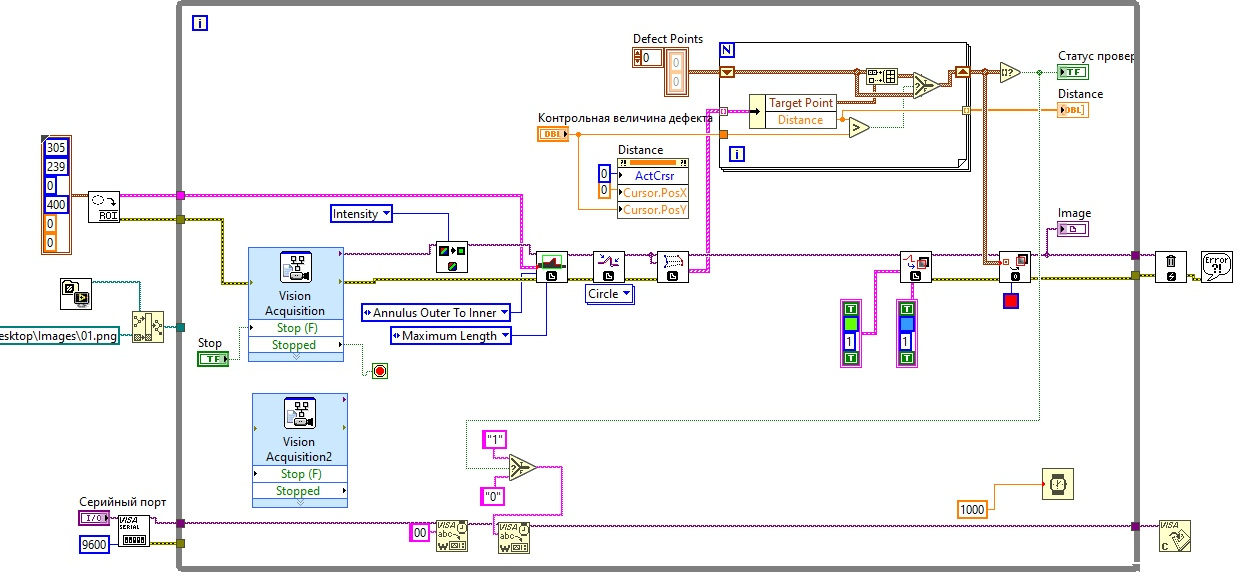
\includegraphics[width=\textwidth]{media/ict2/image182}
	\caption*{14-сурет. Виртуалды аспаптың блок-сұлбасы}
\end{figure}

\begin{figure}[H]
    \centering
    \begin{subfigure}[t]{0.49\textwidth}
        \centering
        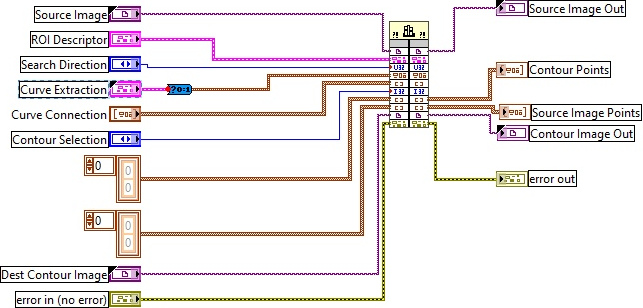
\includegraphics[width=\textwidth]{media/ict2/image183}
        \caption*{}
    \end{subfigure}
    \begin{subfigure}[t]{0.49\textwidth}
        \centering
        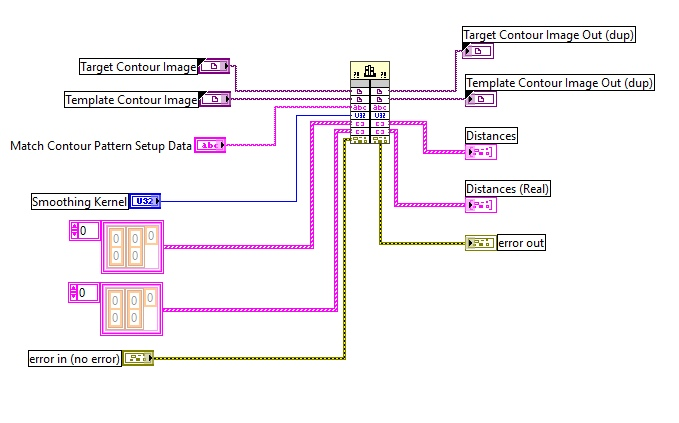
\includegraphics[width=\textwidth]{media/ict2/image184}
        \caption*{}
    \end{subfigure}
    \begin{subfigure}[t]{0.6\textwidth}
        \centering
        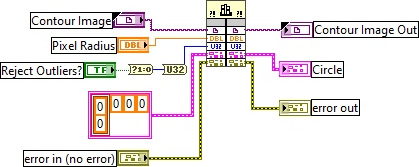
\includegraphics[width=\textwidth]{media/ict2/image185}
        \caption*{}
    \end{subfigure}
    \caption*{15 сурет. IMAQ Extract Contour VI, IMAQ Fit Contour VI, IMAQ Compute Contour Distances VI қосалқы құралдардың блок- сұлбалары}
\end{figure}

\begin{multicols}{2}
Осылайша, жоғарыда сипатталған алгоритмдер блок схемаға кіретін бейненің
контурын талдайды. Блок схеманың шығуына салынған контурлары,
контурлардың сәйкессіздік шамасы және логикалық мәні бар алынған бейне
шығарылады. Нақ осы логикалық мән бұйымның мәртебесін анықтайды және
микроконтроллерге жіберіледі.

Микроконтроллер осы қисынды мәндерді қабылдайды және оларды төлемнің
сандық шығуларындағы басқару сигналдарына түрлендіреді.
Микроконтроллердің осы шығу жолдарына әртүрлі роботталған жабдықтарды
қосу мүмкіндігі бар. Бұл жобада шығу жолдарындағы сигналдың болуы
жарықдиодтардың көмегімен көрсетіледі. Қызыл жарық диоды бұйымның
тексеруден өтпегенін және ақау болып табылатынын хабарлайды. Жасыл жарық
диоды өнімнің талаптарға сай келетінін көрсетеді.16-суретте
микроконтроллерге жүктелген бағдарламалық код көрсетілген.
\end{multicols}

\begin{figure}[H]
	\centering
	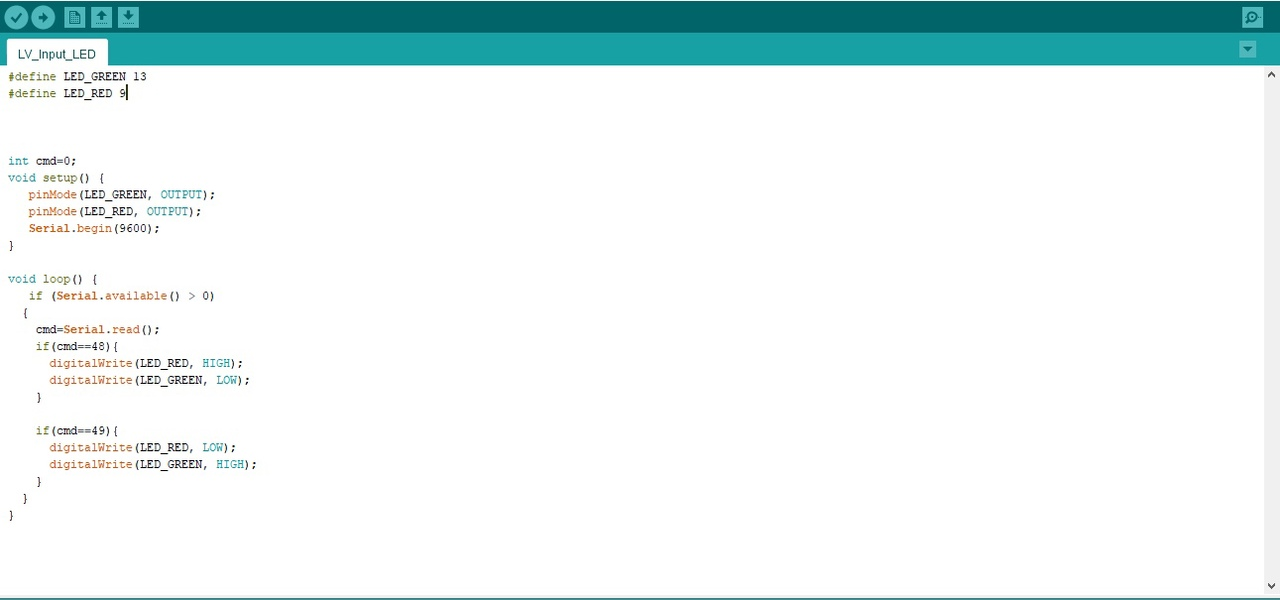
\includegraphics[width=0.8\textwidth]{media/ict2/image186}
	\caption*{16-сурет. Микроконтроллердің программалық коды}
\end{figure}

\begin{multicols}{2}
Сұрыптау және бракқа шығару процестерін автоматтандыру өндірістің сапасы
мен өнімділігін арттыруға мүмкіндік береді. Бұл үшін жасанды интеллект
және техникалық көзқарас технологиялары пайдаланылады.

LabVIEW компьютерлік технологиялары кейіннен өнеркәсіптік жүйеге
кіріктіре отырып, техникалық көрудің бақылау-өлшеу жүйелерін құру үшін
кең мүмкіндіктерге ие.

Әзірленген роботтандырылған жүйе адамның қатысуынсыз автоматты режимде
өндірісте бұйымдарды сұрыптауға және іріктеуге мүмкіндік береді,
осылайша өндірістік процестің сапасы мен өнімділігін арттырады. Бұл
ретте бұл жүйе бракқа шығару процесінің мониторингін жүзеге асыруға
мүмкіндік береді.

Қорытынды: Сұрыптау және бракқа шығару процестерін автоматтандыру
өндірістің сапасы мен өнімділігін арттыруға мүмкіндік береді. Бұл үшін
жасанды интеллект және техникалық көзқарас технологиялары пайдаланылады.

LabVIEW компьютерлік технологиялары кейіннен өнеркәсіптік жүйеге
кіріктіре отырып, техникалық көрудің бақылау-өлшеу жүйелерін құру үшін
кең мүмкіндіктерге ие.

Әзірленген роботтандырылған жүйе адамның қатысуынсыз автоматты режимде
өндірісте бұйымдарды сұрыптауға және іріктеуге мүмкіндік береді,
осылайша өндірістік процестің сапасы мен өнімділігін арттырады. Бұл
ретте бұл жүйе бракқа шығару процесінің мониторингін жүзеге асыруға
мүмкіндік береді.

{\bfseries Қорытынды}. Сұрыптау және бракқа шығару процестерін
автоматтандыру өндірістің сапасы мен өнімділігін арттыруға мүмкіндік
береді. Бұл үшін жасанды интеллект және техникалық көзқарас
технологиялары пайдаланылады.

LabVIEW компьютерлік технологиялары кейіннен өнеркәсіптік жүйеге
кіріктіре отырып, техникалық көрудің бақылау-өлшеу жүйелерін құру үшін
кең мүмкіндіктерге ие.

Әзірленген роботтандырылған жүйе адамның қатысуынсыз автоматты режимде
өндірісте бұйымдарды сұрыптауға және іріктеуге мүмкіндік береді,
осылайша өндірістік процестің сапасы мен өнімділігін арттырады. Бұл
ретте бұл жүйе бракқа шығару процесінің мониторингін жүзеге асыруға
мүмкіндік береді.
\end{multicols}

\begin{center}
{\bfseries Әдебиеттер}
\end{center}

\begin{references}
1. Скоренко Т. Взгляните на мир глазами робота: как устроено «машинное
зрение». URL:\\
\href{https://www.popmech.ru/technologies/238704-glazami-robota-chtotakoe-mashinnoe-zrenie/}{https://www.popmech.ru}. -Дата обращения: 06.01.2025.

2. Куприянов Д., Мусалимов В., Монахов Ю. Адаптивный алгоритм
технического зрения для SLAM систем. Динамика и виброакустика машин:
материалы третьей международной научно-технической конференции, 29 июня
- 01 июля 2016 г. -Самара: Самарский университет, 2016. -- C.250-251.
ISBN 978-5-7883-1088-6.

3. Махов В., Широбоков В., Закутаев А. Построение систем технического
зрения на базе компьютерных технологий National Instruments // Control
Engineering Россия.- 2018.- №4 (76). - С.62-69.

4. Лайонс, Р. Цифровая обработка сигналов: 2-е изд. -- М.: ООО
"Бином-Пресс", 2011.176 с. ISBN 978-5-9518-0446-4.

5. Рудаков П.И., Сафонов В.И. Обработка сигналов и изображений matlab --
под общ. ред. Потемника В.Г. М.: Диалог-МИФИ, 2000. -416 с. - (Пакеты
прикладных программ; Кн.2). - ISBN 5-86404-144-0 (Кн.2).

6. KR 40 PA.
URL: \href{https://www.kuka.com/en-de/products/robot-systems/industrial-robots/kr-40-pa.html}{https://www.kuka.com}.-
Дата обращения: 06.01.2025.

7. Bress T. Effective Labview Programming. New York: NTC Press, 2013. -
720 p. ISBN: 978-1-934891-08-7.

8. What Is NI LabVIEW? URL: \href{https://www.ni.com/ru-ru/shop/labview.html}{https://www.ni.com}.-
Дата обращения: 06.01.2025.

9. Kalkman C.J. LabVIEW: A software system for data acquisition, data
analysis, and instrument contro
l//\href{https://link.springer.com/journal/10877}{Journal of Clinical
Monitoring} and Computing.-1995.- Vol.11.-P.51-58.

10. Трэвис Дж. LabVIEW для всех: пер. с англ. М. П. Михеева. -М.: ДМК
Пресс, 2023. - 905 с. ISBN 978-5-89818-491-9.
\end{references}

\begin{center}
{\bfseries References}
\end{center}

\begin{references}
1. Skorenko T. Vzgljanite na mir glazami robota: kak ustroeno «mashinnoe
zrenie». URL:\\
\href{https://www.popmech.ru/technologies/238704-glazami-robota-chtotakoe-mashinnoe-zrenie/}{https://www.popmech.ru}. -Data obrashhenija: 06.01.2025. {[}in Russian{]}

2. Kuprijanov D., Musalimov V., Monahov Ju. Adaptivnyj algoritm
tehnicheskogo zrenija dlja SLAM sistem. Dinamika i vibroakustika mashin:
materialy tret' ej mezhdunarodnoj nauchno-tehnicheskoj\\
konferencii, 29 ijunja - 01 ijulja 2016 g. -Samara: Samarskij
universitet, 2016. -- C.250-251. ISBN 978-5-7883-1088-6. {[}in
Russian{]}

3. Mahov V., Shirobokov V., Zakutaev A. Postroenie sistem tehnicheskogo
zrenija na baze komp' juternyh tehnologij National
Instruments // Control Engineering Rossija.- 2018.- №4 (76). - S.62-69.
{[}in Russian{]}

4. Lajons, R. Cifrovaja obrabotka signalov: 2-e izd. -- M.: OOO
"Binom-Press", 2011.176 s. ISBN 978-5-9518-0446-4. {[}in Russian{]}

5. Rudakov P.I., Safonov V.I. Obrabotka signalov i izobrazhenij matlab
-- pod obshh. red. Potemnika V.G. M.: Dialog-MIFI, 2000. -416 s. -
(Pakety prikladnyh programm; Kn.2). - ISBN 5-86404-144-0 (Kn.2). {[}in
Russian{]}

6. KR 40 PA.
URL: \href{https://www.kuka.com/en-de/products/robot-systems/industrial-robots/kr-40-pa.html}{https://www.kuka.com}.-
Data obrashhenija: 06.01.2025. {[}in Russian{]}

7. Bress T. Effective Labview Programming. New York: NTC Press, 2013. -
720 p. ISBN: 978-1-934891-08-7.

8. What Is NI LabVIEW? URL: \href{https://www.ni.com/ru-ru/shop/labview.html}{https://www.ni.com}.-
Data obrashhenija: 06.01.2025.

9. Kalkman C.J. LabVIEW: A software system for data acquisition, data
analysis, and instrument contro
l//\href{https://link.springer.com/journal/10877}{Journal of Clinical
Monitoring} and Computing.-1995.- Vol.11.-P.51-58.

10. Трэвис Дж. LabVIEW для всех: пер. с англ. М. П. Михеева. -М.: ДМК
Пресс, 2023. - 905 с. ISBN 978-5-89818-491-9.
\end{references}

\begin{authorinfo}
\hspace{1em}\emph{{\bfseries Сведения об авторах}}

Нурахметов Б.К.- д.т.н., профессор, Алматинский технологический
университета, Алматы, Казахстан, e-mail: \\b.nurakhmetov@mail.ru;

Жумашева Ж.Т. - кандидат технических наук, доцент, КазНУ им. аль-Фараби,
Алматы, Казахстан, e-mail: \\Zhadyra\_14@mail.ru;

\hspace{1em}\emph{{\bfseries Information about the authors}}

Nurakhmetov B.K. -- doctor of technical sciences,Professor, Almaty
Technological University, Almaty, Kazakhstan, e-mail: b.nurakhmetov@mail.ru;

Zhumasheva Zh.T.-PhD, Associate Professor of Al-Farabi Kazakh National
University, Almaty, Kazakhstan, e-mail:\\ Zhadyra\_14@mail.ru;
\end{authorinfo}
